\section{API}

A \textit{Web} API é composta por 2 módulos principais (API e Service) e um conjunto de módulos auxiliares. Enquanto que a API é lida com pedidos e respostas HTTP e o serviço é responsável por implementar a lógica do sistema, existem ainda os repositórios (sendo que cada um se responsabiliza por implementar a sua própria lógica de acesso a base de dados) e o índice de imagens (responsável por tratar todas as operações associadas a imagens).

\begin{figure}[h]
	\centering
	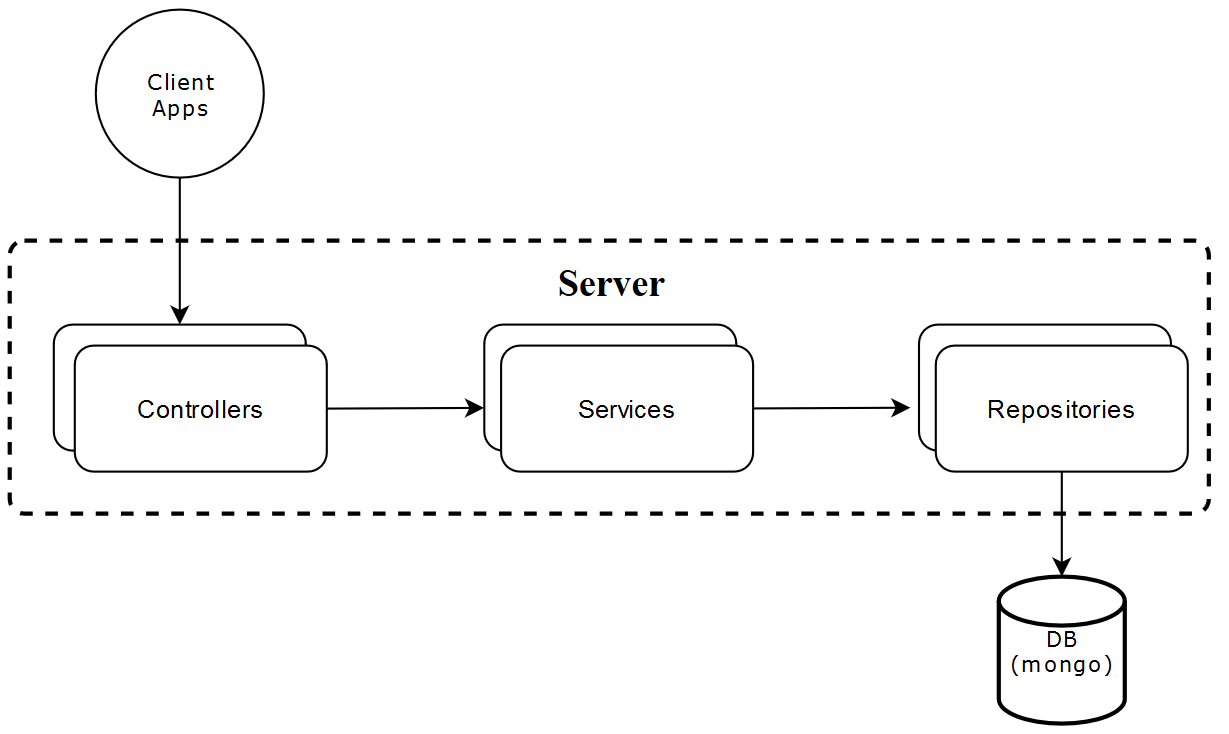
\includegraphics[scale=.50]{api_architeture}
	\caption{Diagrama de arquitetura da API}
\end{figure}

\subsection{Server}
(todo server)

\subsection{API}
(todo api)

(fazer tabela com endpoints)

\subsection{Serviço}
(todo service)

\subsection{Repositórios e acesso a base de dados}
(todo repositories and base repository)

\subsection{Base de Dados}

\subsection{Autenticação}

\subsection{Imagens}
(todo pictures)

\subsection{Documentação e definição da API}